\documentclass{beamer}
\usepackage{tikz}
\usepackage[all]{xy}
\usepackage{amsmath,amssymb}
\usepackage{hyperref}
\usepackage{graphicx}
 
\DeclareMathOperator*{\argmin}{arg\,min}
\DeclareMathOperator*{\Lik}{Lik}
\DeclareMathOperator*{\PoissonLoss}{PoissonLoss}
\DeclareMathOperator*{\Peaks}{Peaks}
\DeclareMathOperator*{\Segments}{Segments}
\DeclareMathOperator*{\argmax}{arg\,max}
\DeclareMathOperator*{\maximize}{maximize}
\DeclareMathOperator*{\minimize}{minimize}
\newcommand{\sign}{\operatorname{sign}}
\newcommand{\RR}{\mathbb R}
\newcommand{\ZZ}{\mathbb Z}
\newcommand{\NN}{\mathbb N}
\newcommand{\z}{$z = 2, 4, 3, 5, 1$} 

\newcommand{\algo}[1]{\textcolor{#1}{#1}}
\definecolor{PDPA}{HTML}{66C2A5}
\definecolor{CDPA}{HTML}{FC8D62}
\definecolor{GPDPA}{HTML}{4D4D4D}

% Set transparency of non-highlighted sections in the table of
% contents slide.
\setbeamertemplate{section in toc shaded}[default][100]
\AtBeginSection[]
{
  \setbeamercolor{section in toc}{fg=red} 
  \setbeamercolor{section in toc shaded}{fg=black} 
  \begin{frame}
    \tableofcontents[currentsection]
  \end{frame}
}

\begin{document}

\title{Neural networks for imbalanced classification: proposed AUM loss with mlr3torch in R}

\author{
  Toby Dylan Hocking\\
  Professeur Agrégé, 2024--present,\\
  Département d'Informatique\\
  Université de Sherbrooke\\
  toby.dylan.hocking@usherbrooke.ca\\
  toby.hocking@r-project.org\\
}

\maketitle

\section{Unbalanced classification, AUC, and proposed AUM}

\begin{frame}
  \frametitle{Learning two different functions using two data sets}
  Figure from chapter by Hocking TD, \textit{Introduction to machine
    learning and neural networks} for book \textit{Land Carbon Cycle
    Modeling: Matrix Approach, Data Assimilation, and Ecological
    Forecasting} edited by Luo Y (Taylor and Francis, 2022).
  \begin{center}
  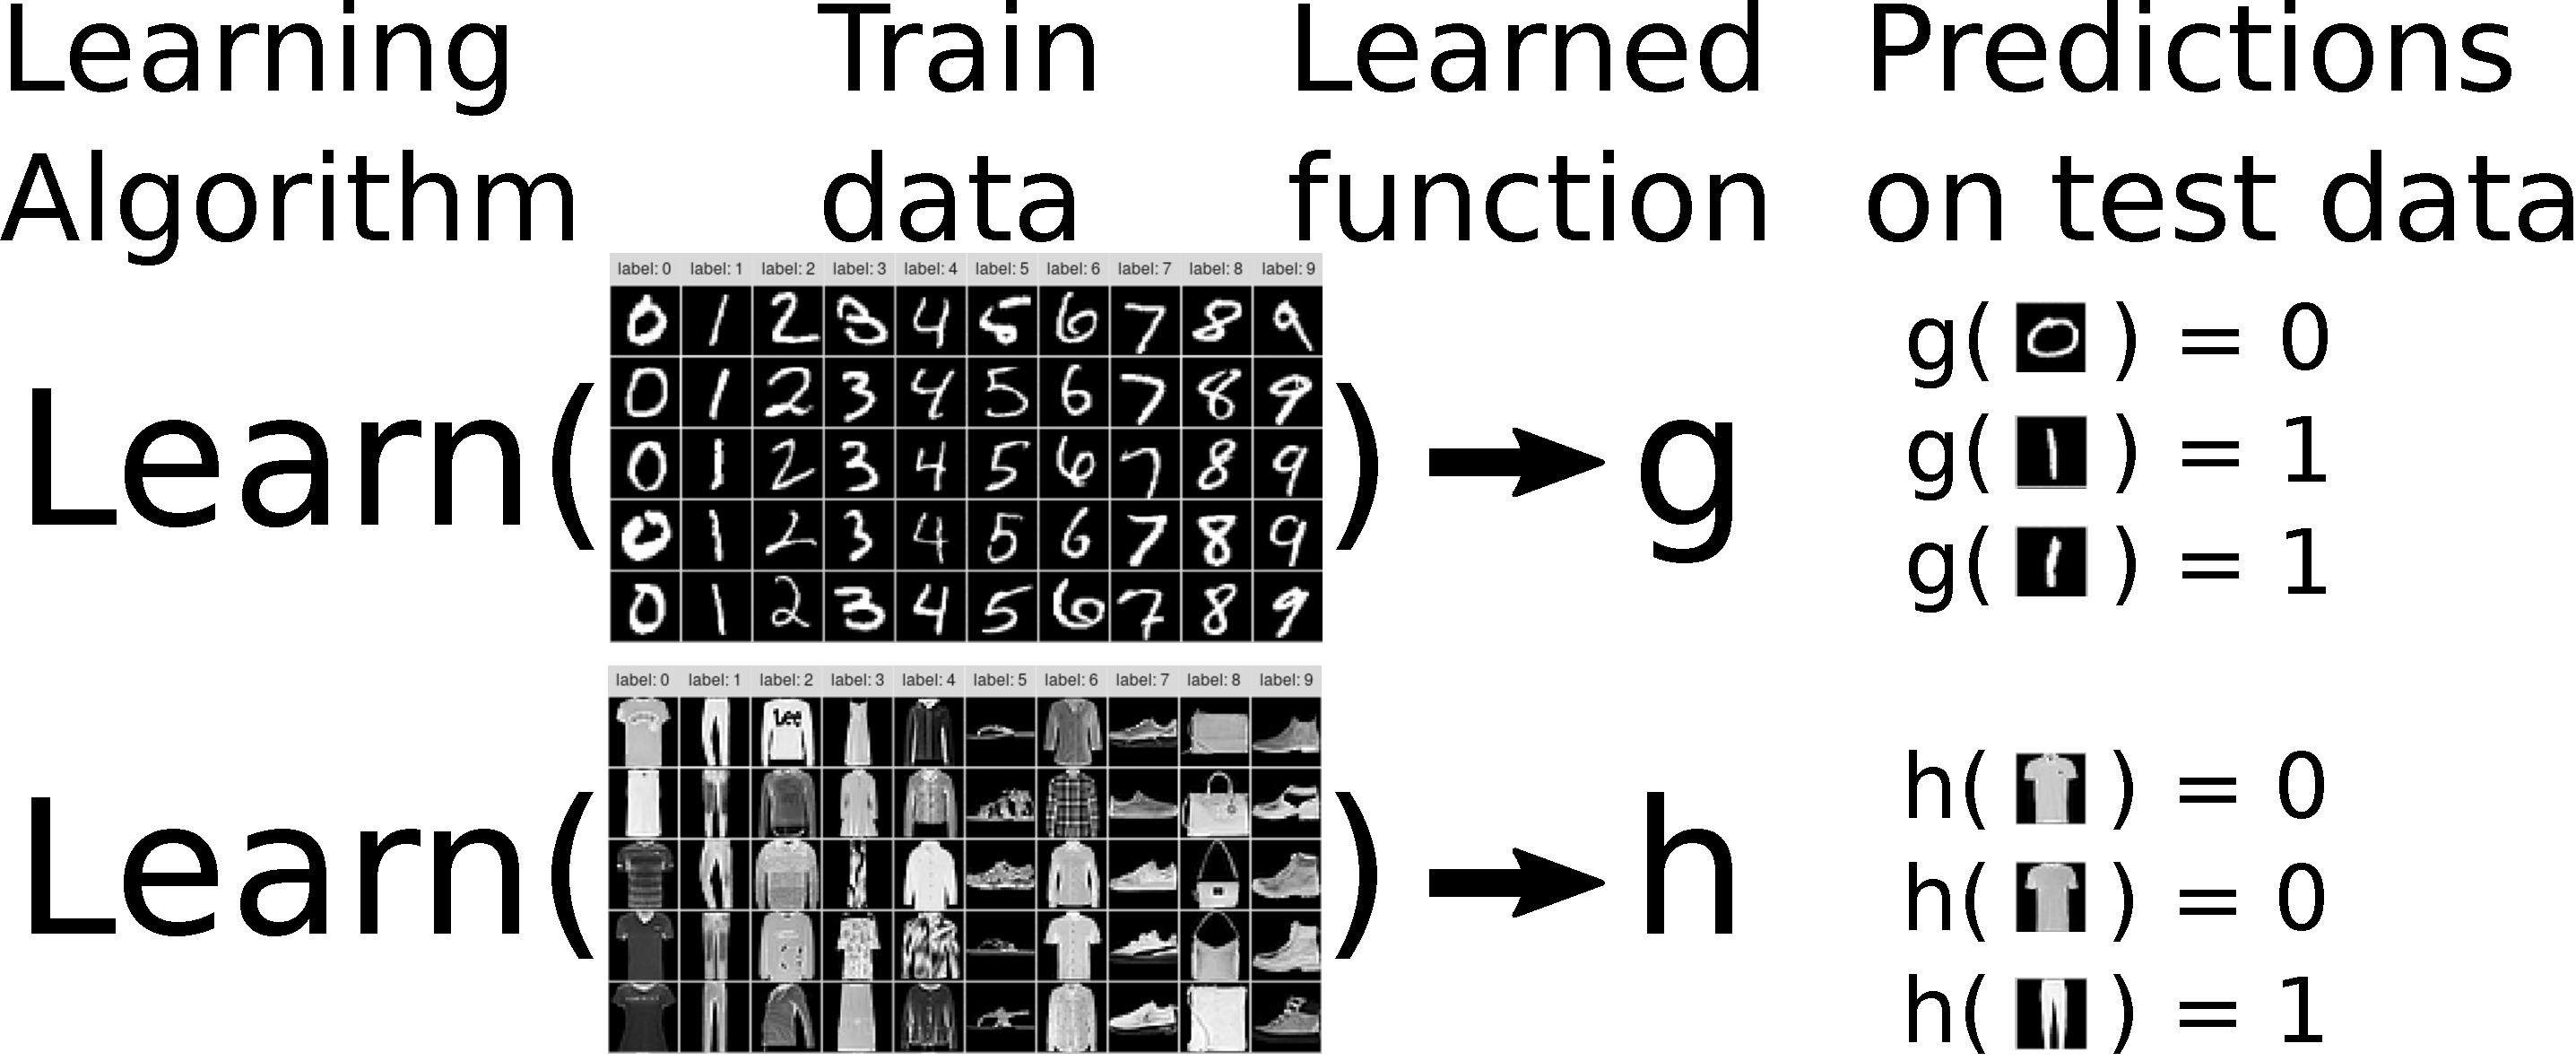
\includegraphics[width=\textwidth]{drawing-mnist-train-test}
\end{center}
\begin{itemize}
\item Ten classes are equally distributed in these data (10\% of each,
  balanced labels).
\item What happens if there are 91\% of one class, and 1\% of each of
  the other 9 classes? (unbalanced labels)
\end{itemize}
\end{frame}

\begin{frame}
  \frametitle{How to deal with class imbalance?}
  \begin{itemize}
  \item In binary classification, standard learning algorithms can yield sub-optimal prediction accuracy if train data have imbalanced labels.
  \item Predicting childhood autism (Lindly \emph{et al.}), 3\% autism, 97\% not.
  \item Predicting presence of trees/burn in satellite imagery
    (Shenkin \emph{et al.}, \emph{Thibault} \emph{et al.}), small
    percent of trees in deserts of Arizona, small percent of burned
    area out of total forested area in Quebec.
  \item Predicting fish spawning habitat in sonar imagery (Bodine
    \emph{et al.}), small percent of suitable spawning habitat, out of
    total river bed.
  \item How do we adapt our learning algorithm, to handle the class
    imbalance? Re-weighting loss? Over/under-sampling?
  \item \alert{New AUM loss
      for optimizing ROC curve.}
  \end{itemize}
\end{frame}

\begin{frame} \frametitle{ROC curves: fair comparison with different
    default FPR} \parbox{0.65\textwidth}{
    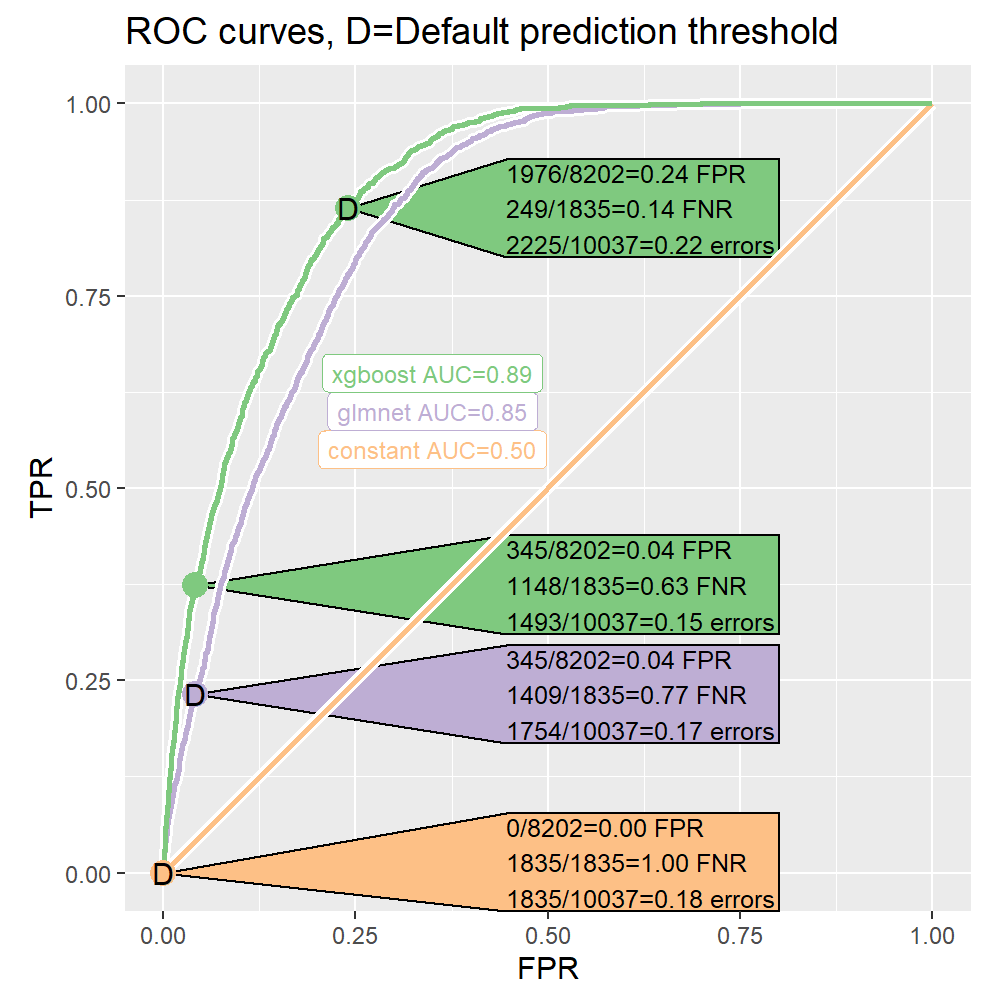
\includegraphics[width=0.65\textwidth]{figure-batchtools-expired-earth-roc}
  } \parbox{0.3\textwidth}{ROC=\\Receiver\\ Operating\\ Characteristic\\ curves
    show FPR, TPR for all cut points of the predicted probability.
  }
  \begin{itemize}
  \item Imbalanced labels: 18\% positive, 82\% negative.
  \item At defaults (D), glmnet has fewer errors (misleading).
  \item At FPR=4\%, xgboost has fewer errors (fair comparison).
  \end{itemize}
\end{frame}

\begin{frame}
  \frametitle{Comparing AUM with weighted logistic loss}
  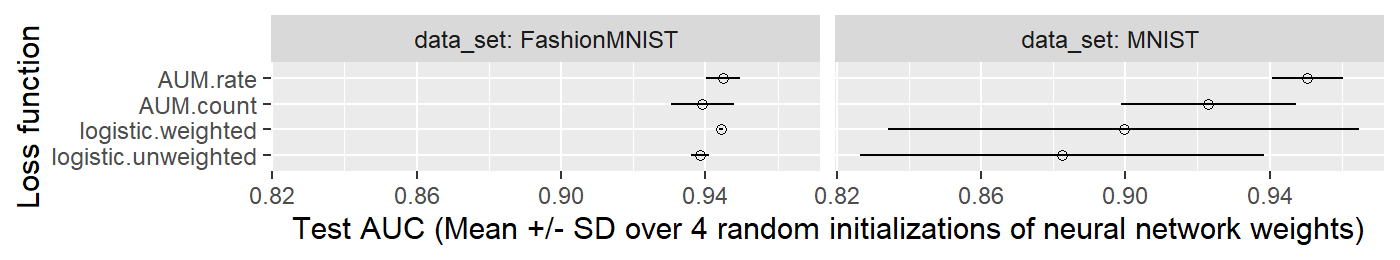
\includegraphics[width=\textwidth]{figure-aum-neural-networks-test-auc}
  Hillman and Hocking, \emph{Journal of Machine Learning Research} 2023.
  \begin{itemize}
  \item Two image classification data sets.
  \item LeNet5 convolutional neural network, batch size 1000.
  \item Step size from $10^{-4}$ to $10^2$ (keep best).
  \item AUM rate uses Area Under Min of FPR/FNR, more accurate in
    these data than AUM count (FP/FN totals), .
  \item logistic unweighted is usual binary cross-entropy loss (uniform weight=1 for each sample). 
  \item for logistic weighted, we compute class frequencies, $n_1=\sum_{i=1}^N I[y_i=1]$ and $n_0$ similar; then weights are $w_i=1/n_{y_i}$ so that total weight of positive class equals total weight of negative class.
  \end{itemize}
\end{frame}

\section{Basics of neural networks with torch in R}

\begin{frame}
  \frametitle{Advantages of torch}
  library(torch) in R provides two key features:
  \begin{itemize}
  \item Automatic gradient computation (auto-grad), which makes it
    easy to implement neural network learning, after having defined
    the network structure and loss function.
  \item Easy speedups using GPUs (if your model and data can fit into
    GPU memory).
  \item Same features as python version of torch, but with less
    documentation and example code.
  \end{itemize}
\end{frame}

\begin{frame}
  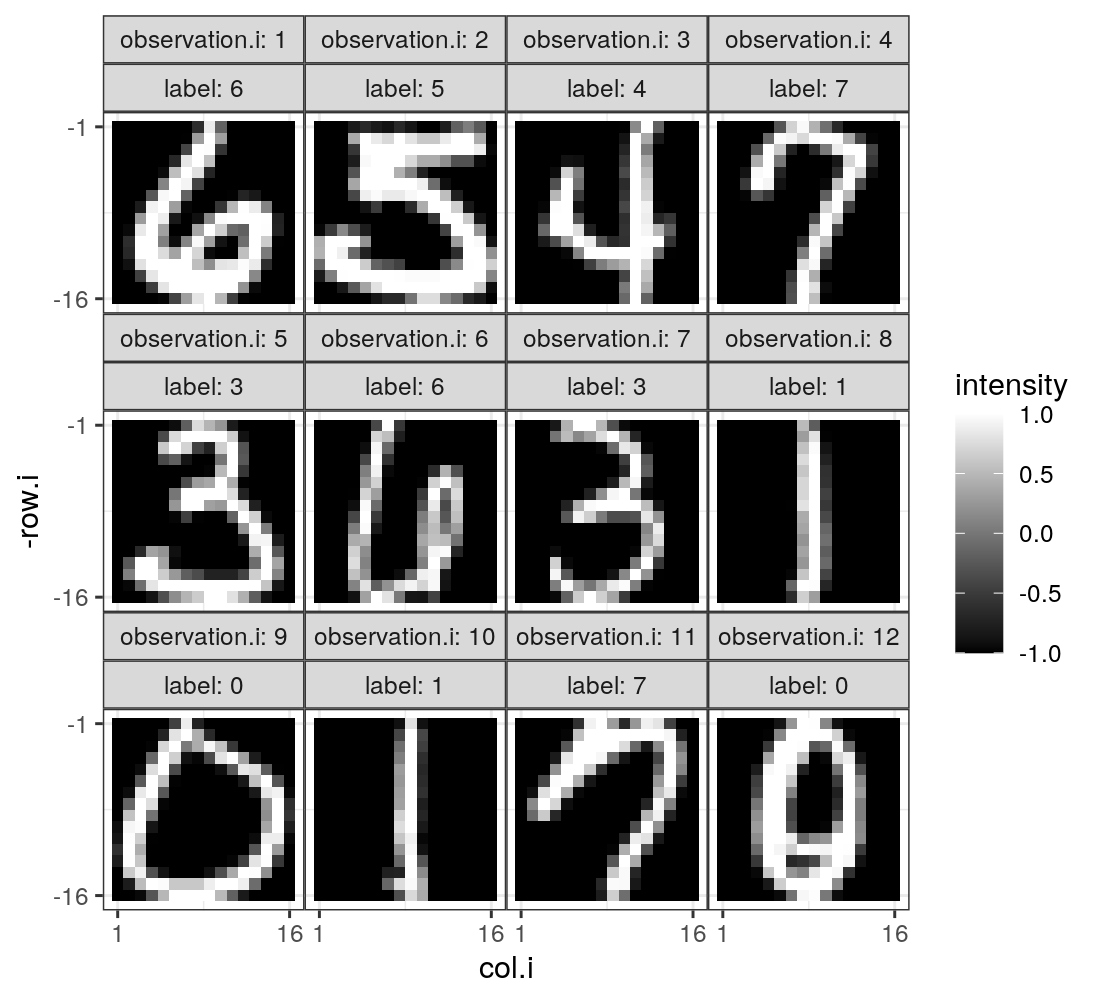
\includegraphics[height=\textheight]{figure-validation-loss-digits}
\end{frame}

\begin{frame}[fragile]
  \frametitle{Representation of digits in CSV}

  \begin{itemize}
  \item Each image/observation is one row.
  \item First column is output/label/class to predict.
  \item Other 256 columns are inputs/features (pixel intensity
    values).
  \end{itemize}
 Data from {\scriptsize \url{https://web.stanford.edu/~hastie/ElemStatLearn/datasets/zip.train.gz}}

\begin{verbatim}
 1:  6 -1 -1  ... -1.000 -1.000   -1
 2:  5 -1 -1  ... -0.671 -0.828   -1
 3:  4 -1 -1  ... -1.000 -1.000   -1
 4:  7 -1 -1  ... -1.000 -1.000   -1
 5:  3 -1 -1  ... -0.883 -1.000   -1
 6:  6 -1 -1  ... -1.000 -1.000   -1
...
\end{verbatim}

Demo: reading CSV, plotting digits, \url{https://github.com/tdhock/2023-res-baz-az/blob/main/2023-04-19-deep-learning.Rmd}
  
\end{frame}

\begin{frame}[fragile]
  \frametitle{Converting R data to torch tensors}
Use array function with all columns except first as data.  
\begin{verbatim}
zip.dt <- data.table::fread("zip.train.gz")
zip.X.array <- array(
  data = unlist(zip.dt[,-1]),
  dim = c(nrow(zip.dt), 1, 16, 16))
zip.X.tensor <- torch::torch_tensor(zip.X.array)
zip.y.tensor <- torch::torch_tensor(
  zip.dt$V1+1L, torch::torch_long())
\end{verbatim}
Need to specify dimensions of input/X array:
\begin{itemize}
\item Observations: same as the number of rows in the CSV table.
\item Channels: 1 (greyscale image, would be 3 for RGB image).
\item Pixels wide: 16.
\item Pixels high: 16.
\end{itemize}
For output/y need to add 1 in R, and specify long int type.
\end{frame}

\begin{frame}
  \frametitle{Network diagram for linear model with 10 inputs/features}
  Neural network
  diagrams show how each unit (node) is computed by applying the
  weights (edges) to the values of the units at the previous layer.
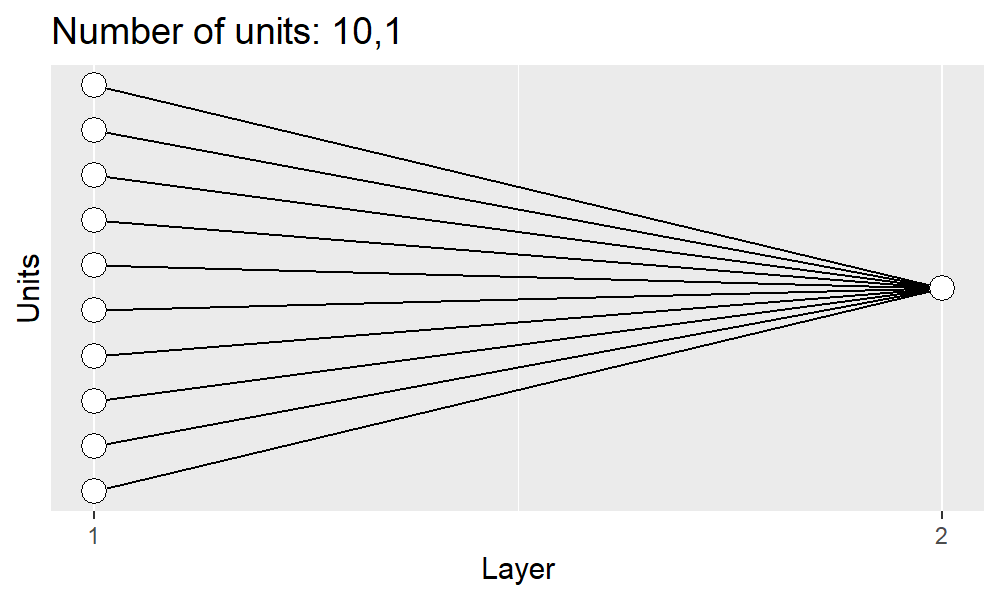
\includegraphics[width=\textwidth]{figure-architecture-linear}
\end{frame}

\begin{frame}[fragile]
  \frametitle{Linear model R code}
\begin{verbatim}
n.features <- 16*16
n.classes <- 10
linear.model <- torch::nn_sequential(
  torch::nn_flatten(),
  torch::nn_linear(n.features, n.classes))
pred.tensor <- linear.model(zip.X.tensor)
\end{verbatim}

  \begin{itemize}
  \item First layer must specify shape of inputs (here 16x16x1).
  \item \texttt{nn\_flatten} converts any shape to a single dimension
    of units (here, convert each image from 1x16x16-array to 256-vector).
  \item \texttt{nn\_linear} uses all units/features in the previous
    layer (256) to predict each unit in the next layer (10).
  \item There are ten possible classes for an output.
  \end{itemize}

\end{frame}

\begin{frame}[fragile]
\frametitle{Computing loss, gradient, parameter updates}
\begin{verbatim}
loss.fun <- torch::nn_cross_entropy_loss()
loss.tensor <- loss.fun(pred.tensor, zip.y.tensor)
step.size <- 0.1#also known as learning rate.
optimizer <- torch::optim_sgd(
  linear.model$parameters, lr=step.size)
optimizer$zero_grad()
loss.tensor$backward()
optimizer$step()
\end{verbatim}
\begin{itemize}
\item \texttt{loss.fun} is the cross-entropy loss for multi-class
  classification, which is directly optimized/minimized in each
  iteration of the gradient descent learning algorithm.
\item \texttt{optimizer} is the version of the gradient descent learning
  algorithm to use.
\item \texttt{backward} method computes gradients.
\item \texttt{step} method updates model parameters based on gradients.
\end{itemize}
\end{frame}

\begin{frame}[fragile]
  \frametitle{Gradient Descent learning algorithm}
\begin{verbatim}
gradient_descent <- 
  function(index.list, model, n_epochs, gradient.set){
  loss.dt.list <- list()
  for(epoch in seq(1, n_epochs)){
    take_steps(index.list[[gradient.set]], model)
    epoch.loss.dt <- loss_each_set(index.list, model)
    loss.dt.list[[paste(epoch)]] <- 
      data.table(epoch, epoch.loss.dt)
  }
  rbindlist(loss.dt.list)
}
\end{verbatim}
  \begin{itemize}
  \item \verb|take_steps| sub-routine updates model parameters.
  \item \verb|loss_each_set| computes loss and error rate on gradient set
    and held-out set.
  \end{itemize}
\end{frame}
 
\begin{frame}
  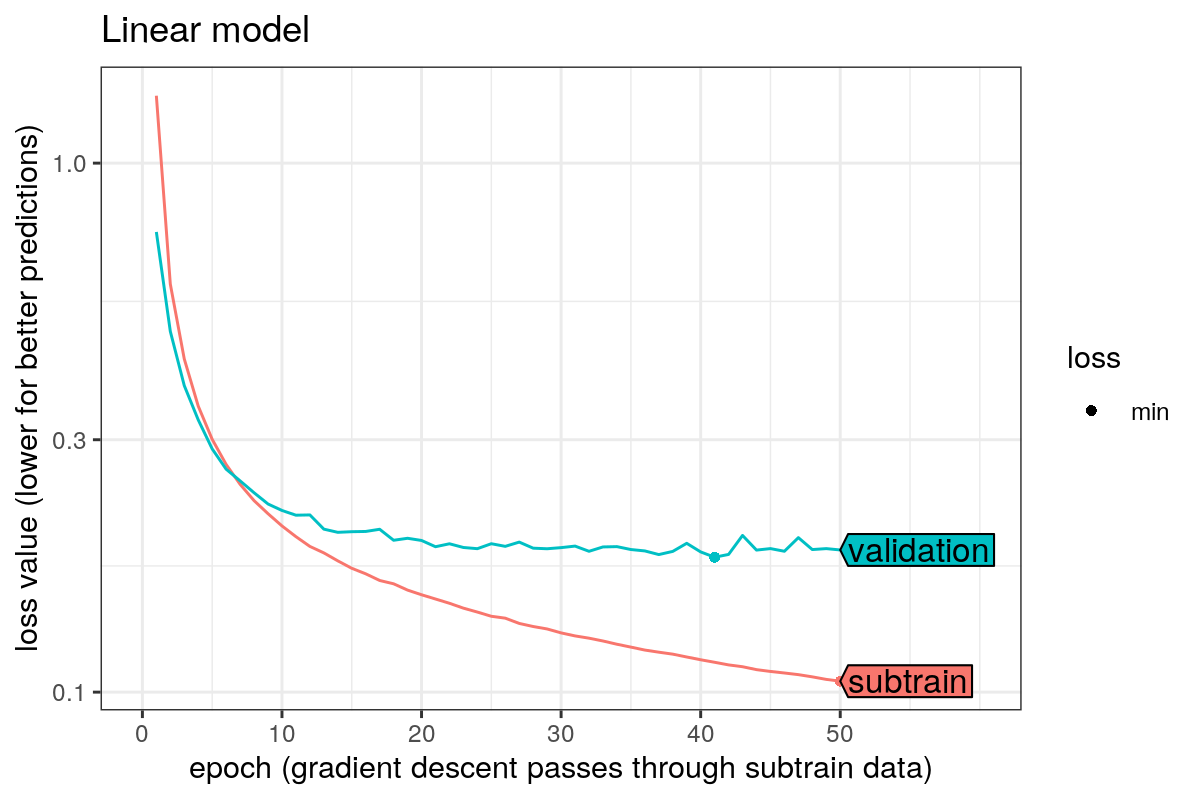
\includegraphics[width=\textwidth]{figure-validation-loss-linear}
  Demo: splitting data, gradient descent loop.
\end{frame}

\begin{frame}
  \frametitle{Network diagram for one hidden layer}
  Neural network
  diagrams show how each unit (node) is computed by applying the
  weights (edges) to the values of the units at the previous layer.
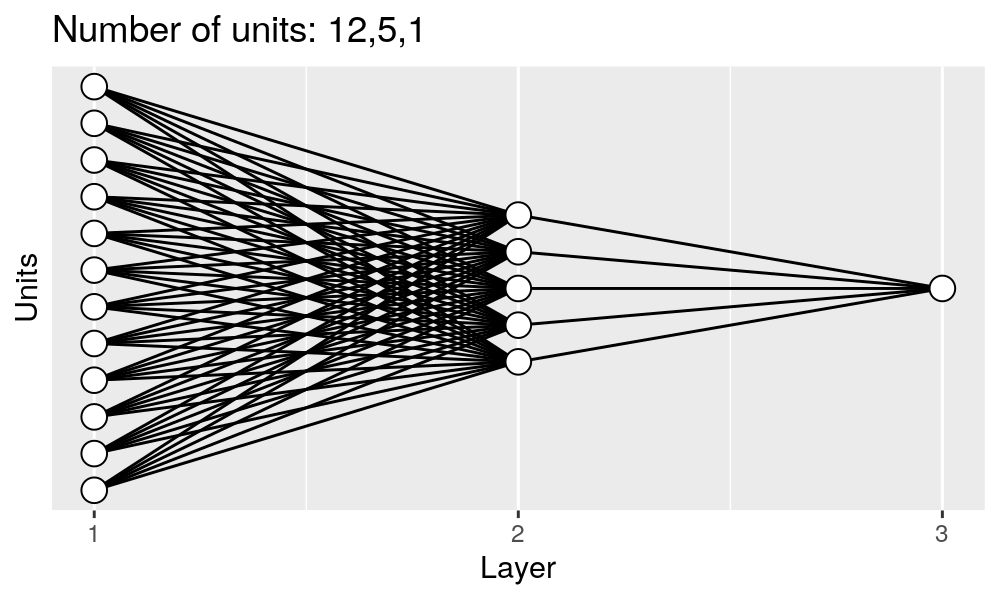
\includegraphics[width=\textwidth]{figure-architecture-oneOut}
\end{frame}
 
\begin{frame}[fragile]
  \frametitle{Dense (fully connected) neural network R code}
\begin{verbatim}
one.hidden.layer <- torch::nn_sequential(
  torch::nn_flatten(),
    torch::nn_linear(n.features, n.hidden.units),
    torch::nn_relu(),
    torch::nn_linear(n.hidden.units, n.classes))
two.hidden.layers <- torch::nn_sequential(
  torch::nn_flatten(),
    torch::nn_linear(n.features, n.hidden.1),
    torch::nn_relu(),
    torch::nn_linear(n.hidden.1, n.hidden.2),
    torch::nn_relu(),
    torch::nn_linear(n.hidden.2, n.classes))
\end{verbatim}
\end{frame}

\begin{frame}
  \frametitle{Network diagram for multiple hidden layers}
  Neural network
  diagrams show how each unit (node) is computed by applying the
  weights (edges) to the values of the units at the previous layer.
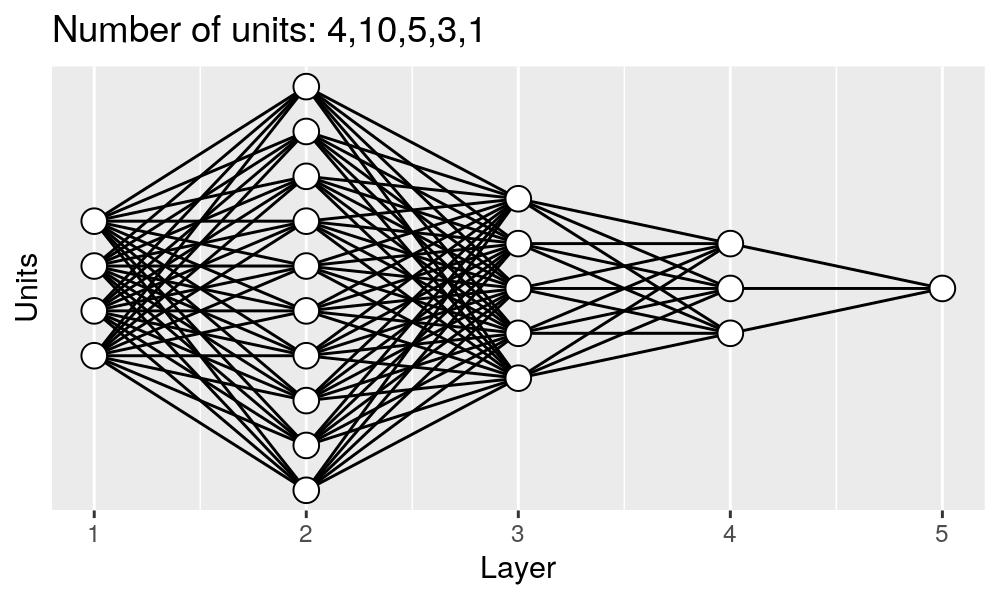
\includegraphics[width=\textwidth]{figure-architecture-fiveLayers}
\end{frame}

\begin{frame}[fragile]
  \frametitle{Use for loop to implement multiple hidden layers}
\begin{verbatim}
new_fully_connected_units <- function(units.per.layer){
  seq.args <- list(torch::nn_flatten())
  for(output.i in seq(2, length(units.per.layer))){
    input.i <- output.i-1
    seq.args[[length(seq.args)+1]] <- torch::nn_linear(
      units.per.layer[[input.i]], 
      units.per.layer[[output.i]])
    if(output.i<length(units.per.layer)){
      seq.args[[length(seq.args)+1]] <- torch::nn_relu()
    }
  }
  do.call(torch::nn_sequential, seq.args)
}
\end{verbatim}
  \begin{itemize}
  \item input a vector of units per layer, for example c(256,1000,100,10).
  \item Begin with flatten.
  \item Linear followed by relu in each layer except last.
  \end{itemize}
\end{frame}
 
\begin{frame}
  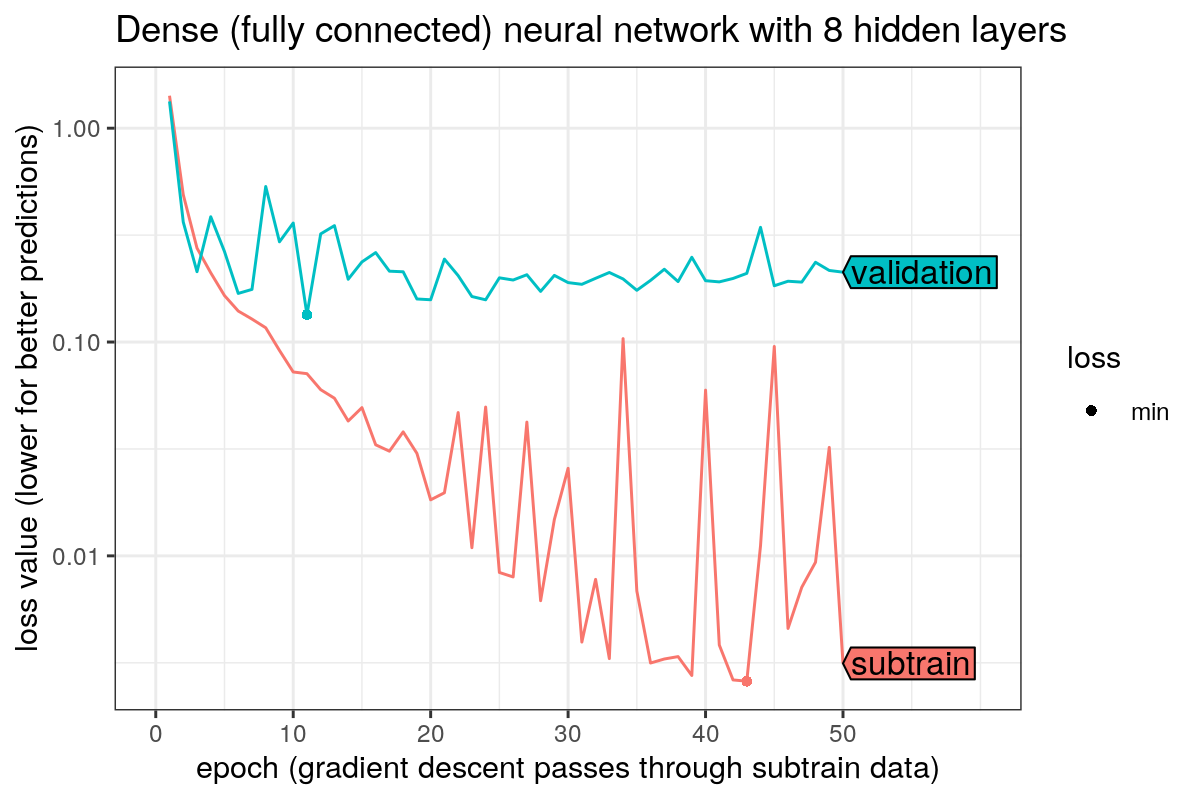
\includegraphics[width=\textwidth]{figure-validation-loss-dense}
\end{frame}
 
\begin{frame}
  \frametitle{2D convolutional kernel for 6x6 pixel image, kernel size=2}
  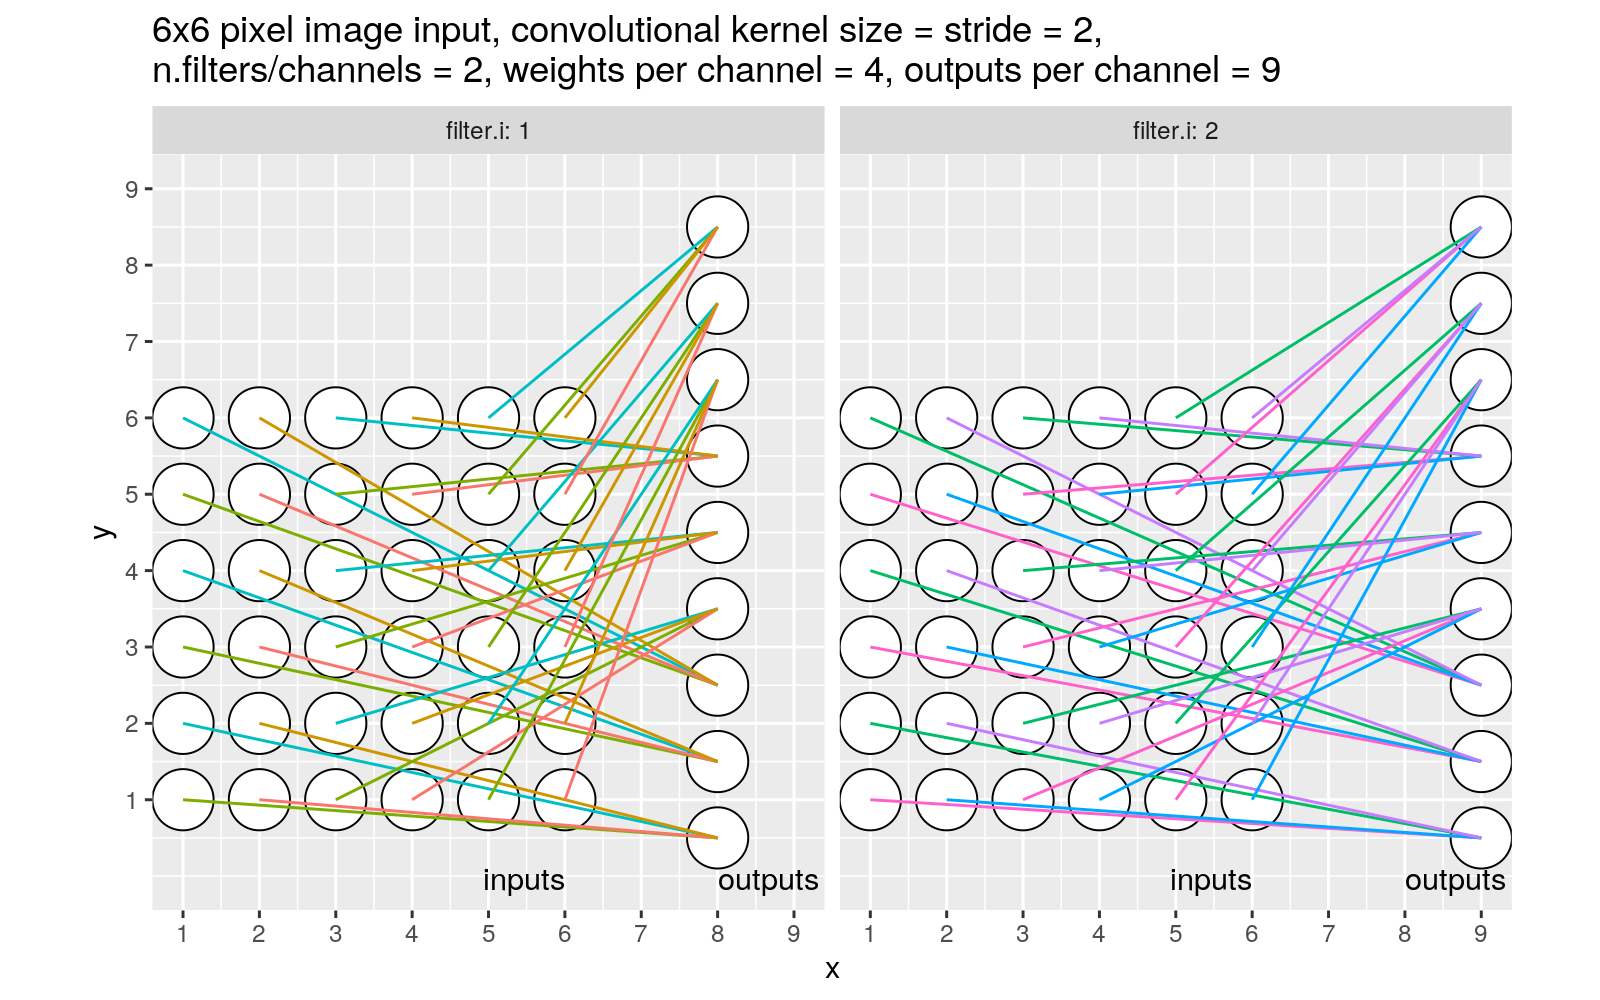
\includegraphics[width=\textwidth]{figure-conv2d-6x6-kernel=2}
\end{frame}

\begin{frame}
  \frametitle{2D convolutional kernel for 6x6 pixel image, kernel size=3}
  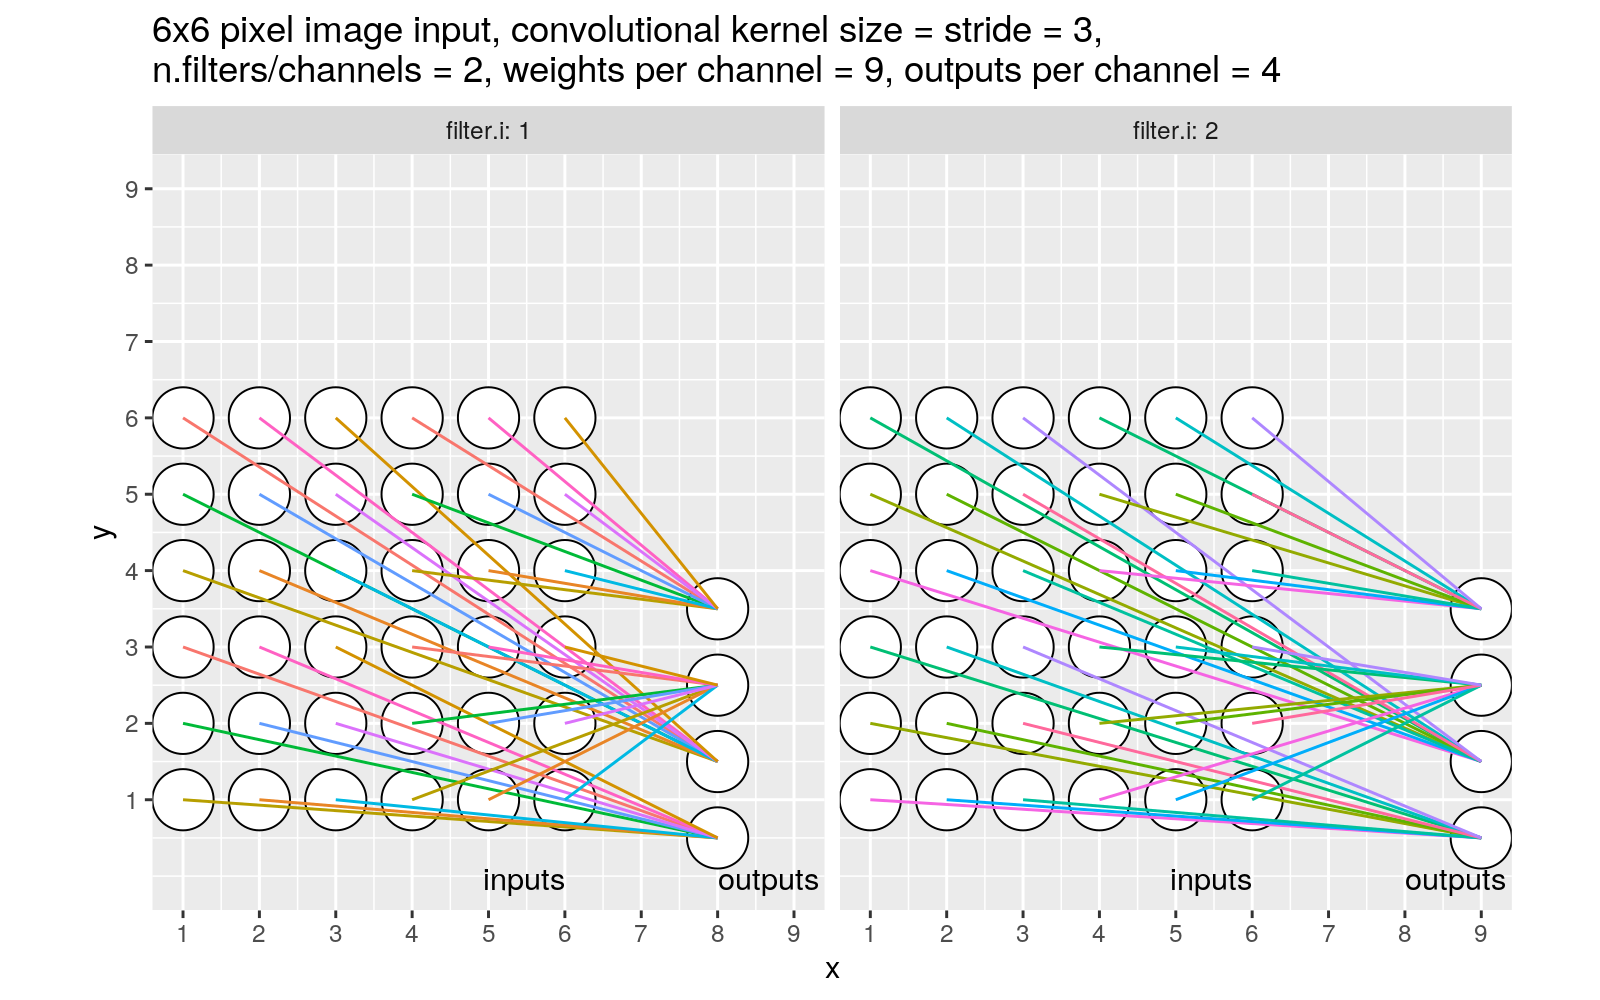
\includegraphics[width=\textwidth]{figure-conv2d-6x6-kernel=3}
\end{frame}

\begin{frame}[fragile]
  \frametitle{Sparse (convolutional) model R code}

\begin{verbatim}
seq2flat <- torch::nn_sequential(
  torch::nn_conv2d(
    in_channels = 1, out_channels = 10, kernel_size = 4),
  torch::nn_relu(),
  torch::nn_flatten(),
  torch::nn_linear(conv.hidden.units, last.hidden.units),
  torch::nn_relu(),
  torch::nn_linear(last.hidden.units, n.classes))
\end{verbatim}

  \begin{itemize}
  \item Two hidden layers: one convolutional, one linear.
  \item Sparse: few inputs are used to predict each unit in
    \texttt{nn\_conv2d}.
  \item Exploits structure of image data to make learning
    easier/faster.
  \end{itemize}

\end{frame}
 
\begin{frame}
  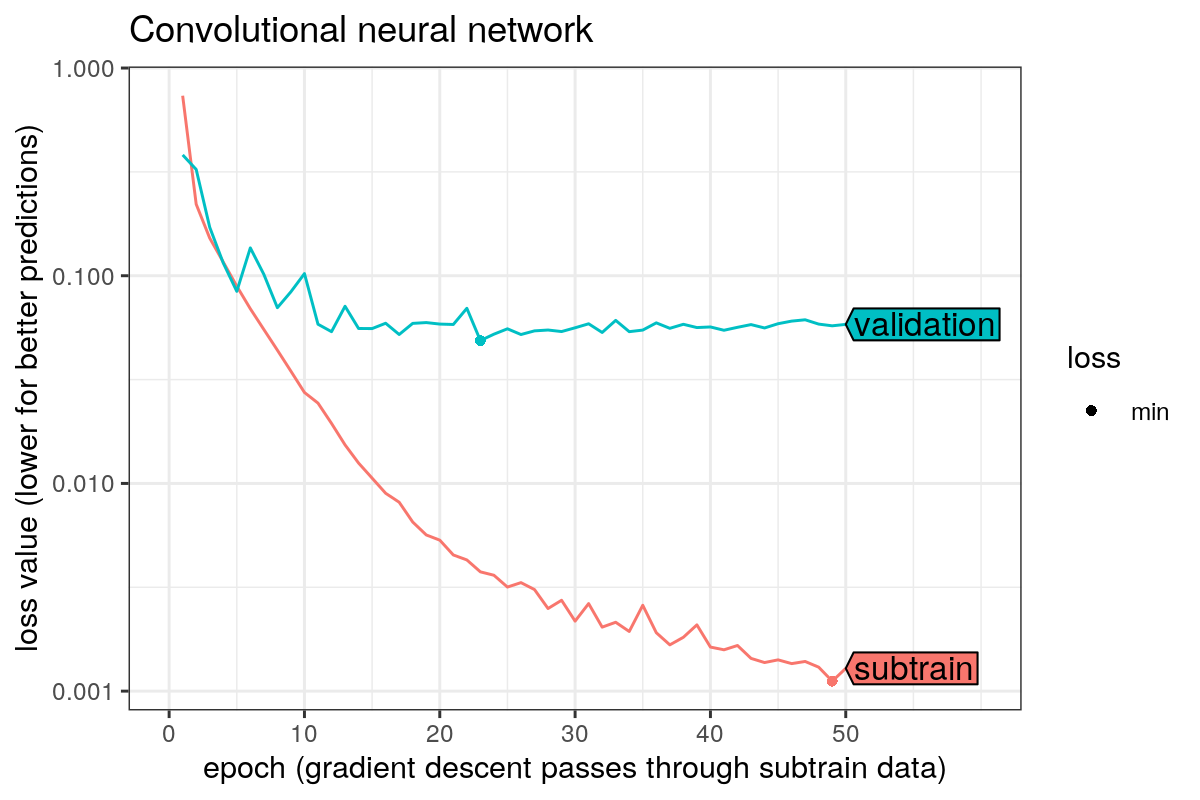
\includegraphics[width=\textwidth]{figure-validation-loss-conv}
\end{frame}
 
\begin{frame}
  \frametitle{Two kinds of cross-validation must be used}
  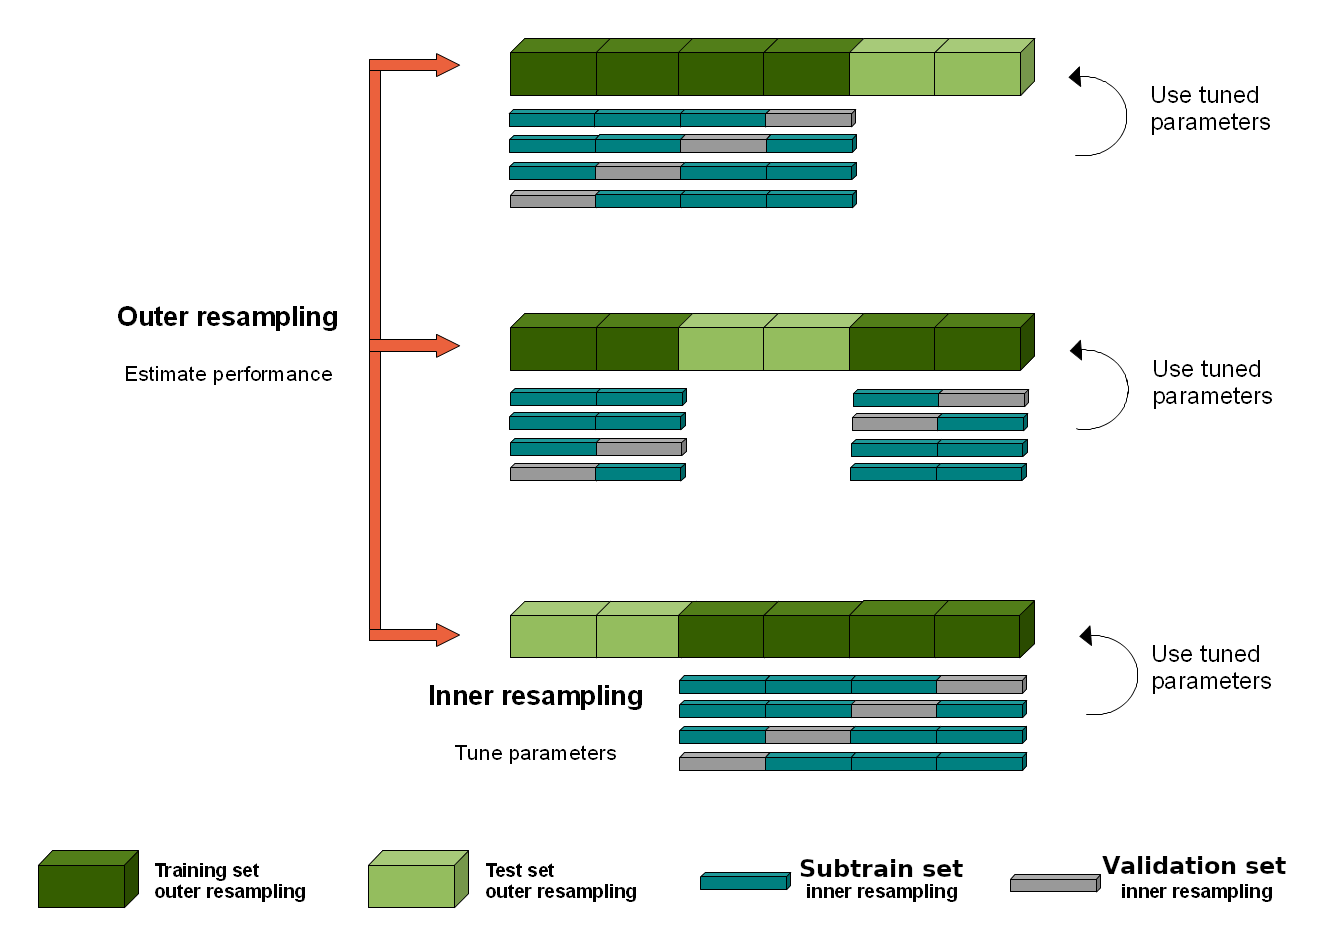
\includegraphics[width=\textwidth]{nested_resampling.png}
  Source: \url{https://mlr.mlr-org.com/articles/tutorial/nested_resampling.html}
\end{frame}

\begin{frame}
  \frametitle{Accuracy rates for each test fold}
  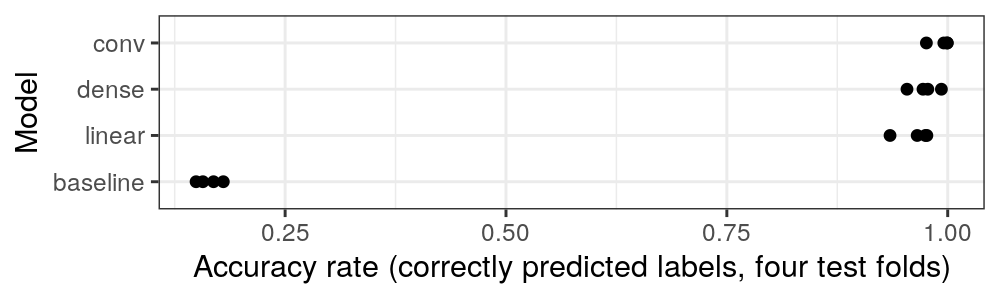
\includegraphics[width=\textwidth]{figure-test-accuracy-baseline}

  \begin{itemize}
  \item Always a good idea to compare with the trivial/featureless baseline model which always
    predicts the most frequent class in the train set. (ignoring all
    inputs/features) 
  \item Here we see that the featureless baseline is much less accurate than the
    three learned models, which are clearly learning something non-trivial.
  \item Code for test accuracy figures:
    \url{https://github.com/tdhock/2023-res-baz-az/blob/main/figure-test-accuracy.R}
  \end{itemize}
\end{frame}
 
\begin{frame}
  \frametitle{Zoom to learned models}
  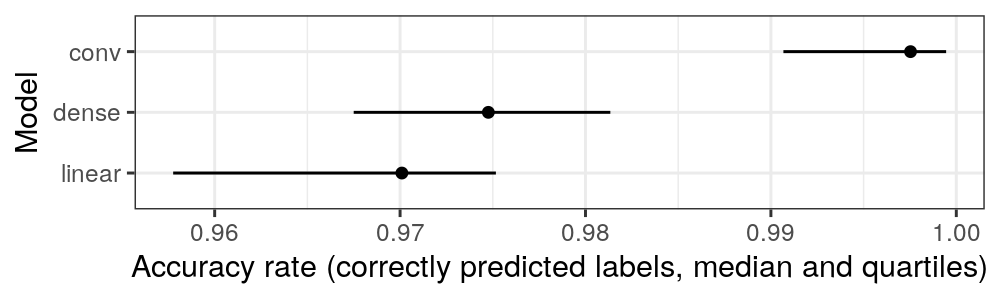
\includegraphics[width=\textwidth]{figure-test-accuracy}
  \begin{itemize}
  \item Dense neural network slightly more accurate
    than linear model, convolutional significantly more
    accurate than others.
  \item Conclusion: convolutional neural network should be preferred
    for most accurate predictions in these data.
  \item Maybe not the same conclusion in other data sets, with the
    same models. (always need to do cross-validation experiments to
    see which model is best in any given data set)
  \item Maybe other models/algorithms would be even more accurate in
    these data. (more/less layers, more/less units, completely
    different algorithm such as random forests, boosting, etc)
  \end{itemize}
\end{frame}

\section{Implementing proposed AUM loss in mlr3torch framework}

\begin{frame}[fragile]
  \frametitle{ROC curve R torch code uses argsort}
\small
  \begin{verbatim}
ROC_curve <- function(pred_tensor, label_tensor){
  sorted_indices = torch_argsort(-pred_tensor$flatten())
... # $cumsum() $diff() etc.
  list(FPR=FPR, FNR=FNR, TPR=1 - FNR, 
    "min(FPR,FNR)"=torch_minimum(FPR, FNR),
    min_constant=torch_cat(c(torch_tensor(-Inf), uniq_thresh)),
    max_constant=torch_cat(c(uniq_thresh, torch_tensor(Inf))))
}
> L <- ROC_curve(torch_tensor(c(2,-3.5,-1,1.5)),
+                torch_tensor(c(0,   0, 1,  1)))
> data.frame(lapply(L, torch::as_array), check.names=FALSE)
  FPR FNR TPR min.FPR.FNR. min_constant max_constant
1 0.0 1.0 0.0          0.0         -Inf         -2.0
2 0.5 1.0 0.0          0.5         -2.0         -1.5
3 0.5 0.5 0.5          0.5         -1.5          1.0
4 0.5 0.0 1.0          0.0          1.0          3.5
5 1.0 0.0 1.0          0.0          3.5          Inf
\end{verbatim}

    \url{https://tdhock.github.io/blog/2024/auto-grad-overhead/}

\end{frame}

\begin{frame}[fragile]
  \frametitle{R code for AUC and proposed AUM both use ROC curve}

  \begin{verbatim}
ROC_AUC <- function(pred_tensor, label_tensor){
  roc = ROC_curve(pred_tensor, label_tensor)
  FPR_diff = roc$FPR[2:N]-roc$FPR[1:-2]
  TPR_sum = roc$TPR[2:N]+roc$TPR[1:-2]
  torch_sum(FPR_diff*TPR_sum/2.0)
}
Proposed_AUM <- function(pred_tensor, label_tensor){
  roc = ROC_curve(pred_tensor, label_tensor)
  min_FPR_FNR = roc[["min(FPR,FNR)"]][2:-2]
  constant_diff = roc$min_constant[2:N]$diff()
  torch_sum(min_FPR_FNR * constant_diff)
}
\end{verbatim}
  Can be used for ROC optimization in binary classification, instead
  of \verb|torch::nn_bce_with_logits_loss|!
\small  \url{https://tdhock.github.io/blog/2024/auto-grad-overhead/}
\end{frame}

\begin{frame}
  \frametitle{Advantages of mlr3 framework}
  \begin{itemize}
  \item Provides standard interface to many popular learning
    algorithms in other R packages. (rpart, glmnet, torch, ...)
  \item Reference implementation of standard algorithms like
    cross-validation.
  \item Makes it easy (no for loop necessary) to setup benchmarks to
    compare prediction accuracy of different algorithms, on different
    data sets, ...
  \item Easy parallelization of benchmarks on super-computer
    clusters. (100--1000x speedups)
  \end{itemize}
\end{frame}

\begin{frame}
  \frametitle{TODO}
  \url{https://tdhock.github.io/blog/2024/mlr3torch/}
\end{frame}

\section{Conclusion}
 
\begin{frame}
  \frametitle{Thanks for participating!}
  \begin{itemize}
  \item Contact: toby.dylan.hocking@usherbrooke.ca, toby.hocking@r-project.org
  \item ROC curves and AUC are used to fairly evaluate binary classification algorithms.
  \item Minimizing proposed AUM loss results in ROC optimization.
  \item Proposed AUM loss can be implemented in torch in R.
  \item Advantages of mlr3 framework include parallelization, simplified code (fewer nested loops).
    
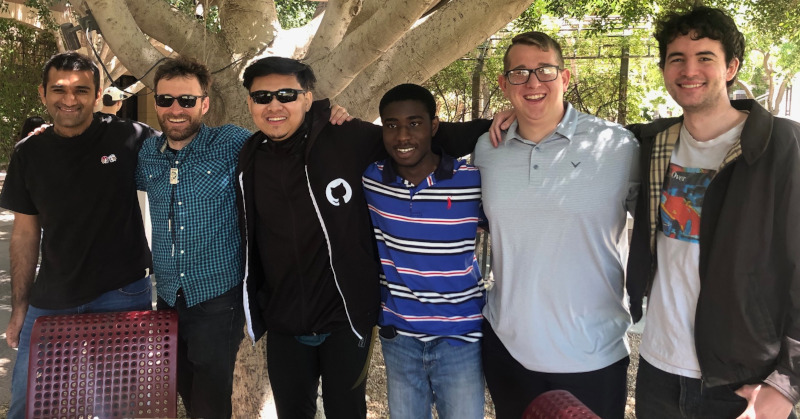
\includegraphics[width=\textwidth]{2023-04-14-ASU-ML-Day}

  \end{itemize}
\end{frame}
 
\begin{frame}
  \frametitle{K-fold cross-validation for model evaluation}
  Is convolutional more accurate on unseen test data?
  
  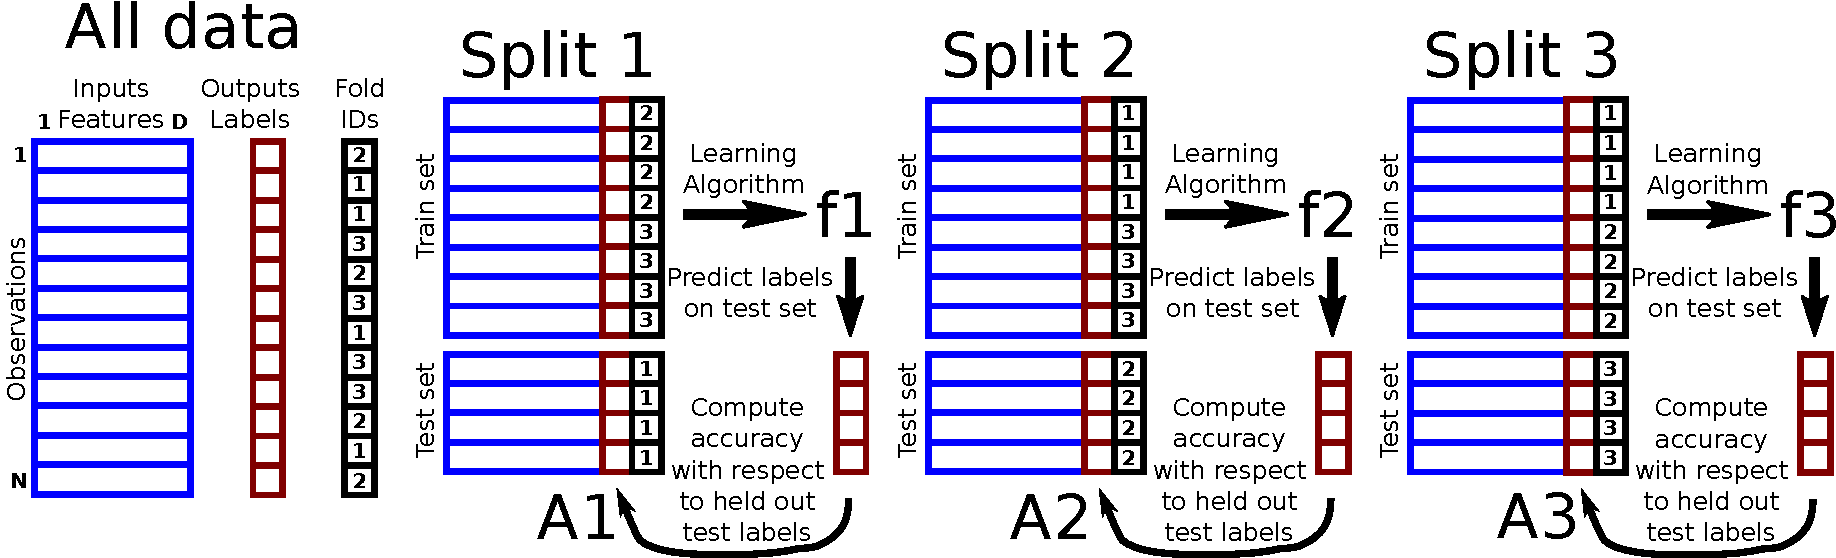
\includegraphics[width=\textwidth]{drawing-cross-validation}
  
  \begin{itemize}
  \item Randomly assign a fold ID from 1 to K to each observation.
  \item Hold out the observations with the Split ID as test set.
  \item Use the other observations as the train set.
  \item Run learning algorithm on train set (including hyper-parmeter
    selection), outputs learned function (f1-f3).
  \item Finally compute and plot the prediction accuracy (A1-A3) with
    respect to the held-out test set.
  \end{itemize}
\end{frame}

\end{document}
